\section{為什麼香港警察近年屢受批評?}

因為不少市民認為警察濫權,執法不公,而且有選擇性。如果警察執法的過程本身不守法,又或執法的嚴謹程度有雙重標準,未能做到一視同仁,就會影響到警察在市民心目中的地位。當警察執法的時候,例如拘捕疑犯或是管理遊行集會秩序,公眾開始質疑他們未必是出於專業判斷而是政治立場。當警察的公信力日漸低落,對政府管治也會構成極壞的影響。

香港警察的公眾形象經歷過不少起跌。回到六、七十年代廉政公署成立前,香港貪污問題十分嚴重,並以警隊尤為明顯。當時幾宗重要的貪污案件,如葛柏案和四大探長等都涉及警隊高層。及後港英政府打擊貪污,警隊和其他紀律部隊的聲譽日益改善。港產片和電視劇集中常見警察類型題材,無論是動作片還是喜劇,均深受觀眾喜愛。

然而,近年警察形象急轉直下。至今,不少市民已慣常對警察醜聞表示幸災樂禍,視警察為公眾笑柄。香港大學民意研究計劃至特區成立以來一直追蹤調查香港人對警務處的滿意度。警務處本來表現不俗,滿意淨值於首十年的平均數為正63.1\%,於二零零七年中更曾一度升至正80.5\%的高點。不過,數據至此便一路往下走,在二零一四年起更大幅下降,並曾於二零一五年初跌至只有正20.9\%的最低點。

\begin{figure}[htbp]
    \centering
    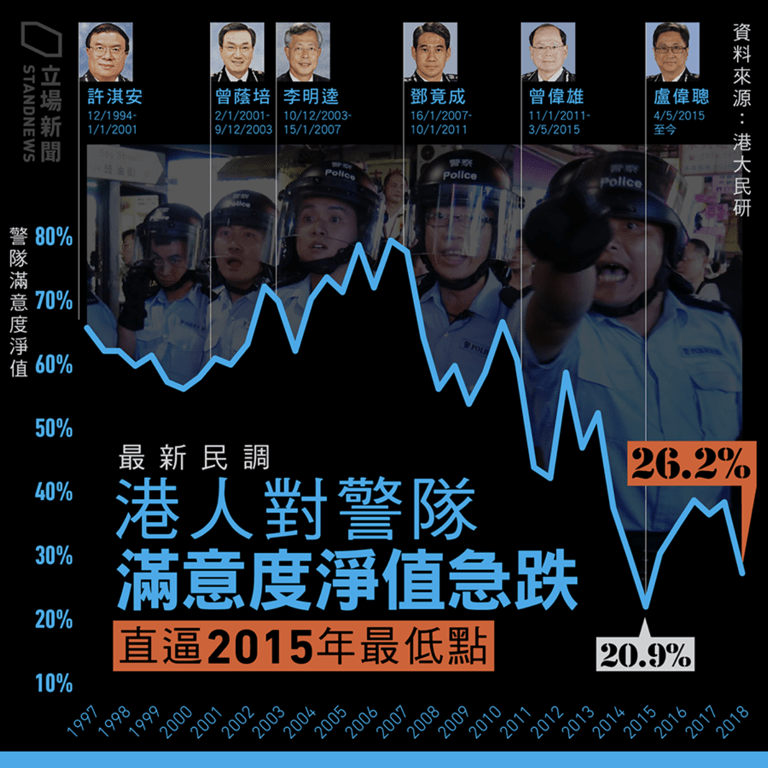
\includegraphics[width=0.7\textwidth]{c30/h-klesson1-047.png}
    \caption{警務處近年變得不受歡迎} 
\end{figure}

冰封三尺亦非一日之寒,輿論批評警察的工作由維持治安變成政權維穩,由來已久。近年警察對遊行集會的管理越來越嚴格,甚至被批為踐踏人權。例如二零一一年時任國務院副總理李克強訪問香港期間,有市民穿著印有「平反六四」字樣的襯衫到他前往家訪的屋苑附近圍觀,隨即被多名沒有出示警察委任證的人員強行押走。有記者上前拍攝,亦被阻擋攝影機鏡頭。警方後來聲稱該市民進入了「核心保安區」,卻遭大律師公會強烈批評香港法律根本沒此概念,就算有保安需要也應按法例設立禁區,警方未能解釋阻擋市民的合法表達權利和記者的採訪自由的依據。

尊重人權一直是香港社會對警察專業操守的主要期望之一。電影中警察拘捕疑犯時的一句「你有權保持緘默」並不只是一句對白,而是說明警察本身也要守法,權力受到限制。然而警察本身不守法的問題日益嚴重,二零一四年佔領運動期間警察的表現嚴重脫離了公眾期望,徹底改變了警察的公眾形象。

在九月二十九日凌晨,也就是佔領運動的第一晚,市民在沒有約定下自發佔領了旺角一帶的街道。警方對此毫無準備,緊急撤離在前線的少數警察,還留下了一輛無人看守的警車。佔領者看到這輛警車不單沒有推翻或破壞,反而把這輛警車用繩圍起來,簡陋地用紙筆留言勸喻其他參與者千萬不要觸碰這輛警車,以示這場運動的文明進步,可見他們當時並沒有視警察為敵,認為警察只是受命工作而被夾在政府和市民中間。

到了十月三日,大批自稱反對佔領人士到旺角包圍和攻擊佔領者,有支持佔領者被打至頭破血流,然而警方卻未有嚴正執法,甚至護送滋事者離開。有反對佔領人士手持水果刀割壞現場帳篷,被傳媒追訪時聲稱「這把刀我到全世界都帶在身上,我很喜歡吃水果,到每個國家都要吃」,卻沒有因為刑事毀壞和在公眾地方管有攻擊性武器而被追究。從當天起各種對不公平執法的質疑,大大打擊了市民對警察專業公正的信心。

佔領者以為警察會保護他們,後面是對香港法治和人權的信任。《基本法》規定香港居民一律平等,沒有說只有支持政府的才會受到保護,反對政府的就不會受到保護。基於對法治的尊重,在香港即使是殺人犯也有人權。法庭可以判犯人坐牢,但在坐牢的過程中仍應被照顧健康和飲食,更不應被隨意毆打。再舉一例,如有食客在餐廳抽煙,則雖然違反了《 吸煙( 公眾衞生) 條例》,卻不等如其他食客可以拿刀砍他,而在場警察更不能因為該食客「違法在先」便就手旁觀。同一邏輯,在旺角的佔領者雖然在參與反對政府的行動,同時認為受襲時警察應該保護他們,本來合理不過。

接下來的「七警案」,則更把公眾對警察的憤怒推向另一個高峰。十月十五日,七名警務人員在金鐘把一名佔領者抬到暗角拳打腳踢,過程剛好被電視新聞拍攝報道。當時佔領者已被反綁雙手,沒有攻擊能力,及後在醫院檢查時發現多處明顯傷痕。涉案七警雖然被停職,卻事發相隔一年後才被落案控告,警方被質疑刻意拖延,警警相衛。雖然七警最終於兩年多後被判罪名成立,但在宣判後卻有支持警察團體和多個警察協會發起集會支持七警。這些集會都沒有按《公安條例》申請公眾集會的「不反對通知書」,不過警方都沒有行動。相對於警察對其他示威活動的嚴格限制,此雙重標準的表現進一步引發公眾對警察互相包庇的質疑。

% \begin{figure}[ht!]
%     \centering
%     \includemedia[
%     width=0.6\linewidth,height=0.45\linewidth,
%     activate=pageopen,
%     flashvars={
%         modestbranding=1  % no YT logo in control bar
%         &autohide=1       % controlbar autohide
%         &showinfo=0       % no title and other info before start
%     }
%     ]{}{https://youtu.be/EAMXIVD8tGs}   % Flash file
%     \caption{「七警案」新聞片段}
% \end{figure}

相對其他社會爭議,警察暴行是最不容辯解的。警察的權力由人民賦予,所以必然有限。警察使用暴力的唯一情況,必然是為了保護其他市民,因而才使用恰如其分的武力把動武者制服。換句話說,當對方沒有攻擊能力的時候,警察的武力必須立即停止,因為從那一刻起他已沒有攻擊其他人的可能。如果繼續動用武力,就是警察暴行和濫用私刑。至於對方之前做了些什麼,有沒有破壞公物或者辱罵警察,與判斷警察暴行本身是沒有任何關係的。這點和平時理解社會爭議總得先分析前因後果很不同,判斷警察暴行時是沒有這個需要的,只要見到有警察攻擊任何沒有還擊能力的人時就可斷定。

很不幸,由於佔領運動中的警察暴行沒有被政府嚴肅正視,更普遍的濫權似乎已變成了警察文化的一部分。在《逃犯條例》修訂引發的衝突中,警察暴行的普遍程度比佔領運動時有過之而無不及。警察於六月十二日的清場行動期間,對在休息並表明行動不便的路人不停噴射胡椒液體驅趕;有已經倒地的示威者被多名警察包圍毆打;警察向示威者發射布袋彈和橡膠子彈時,並沒有按指引射向對方的下半身,更有多宗面部中彈的個案;多名記者在表明身分和沒有阻礙警察行動的情況下,仍然中彈、被毆,或被噴射胡椒液體。凡此種種,已和過去香港警察引以為傲的專業形象相距極遠。公眾普遍質疑因為警察已變成政治打壓的工具,所以政府不再監督警察暴行濫權。

認為政治已經蓋過法治的質疑,並不限於警察本身,也包括對政府公訴制度的不滿。《基本法》第六十三條規定「香港特別行政區律政司主管刑事檢察工作,不受任何干涉。」然而不少輿論認為這條條文只是虛文。和近年遊行集會相關的,就有警察濫捕和律政司濫控的質疑。近年因遊行集會而被捕和被控的人數大幅增加,唯不少最後卻被撤銷起訴,或被法庭判處無罪,政府被評為濫用司法程序以恐嚇示威者。

% \begin{figure}[ht!]
%     \centering
%     \includemedia[
%     width=0.6\linewidth,height=0.45\linewidth,
%     activate=pageopen,
%     flashvars={
%         modestbranding=1  % no YT logo in control bar
%         &autohide=1       % controlbar autohide
%         &showinfo=0       % no title and other info before start
%     }
%     ]{}{https://youtu.be/Vq2FEapkoqA}   % Flash file
%     \caption{《立場新聞》統計佔領運動後的檢控情況}
% \end{figure}

對檢控工作未能做到公平公正的質疑,自特區成立以來已多次出現,當中以一九九八年的胡仙案為第一例。案件原為星島集團旗下報章被揭發誇大發行量,詐騙廣告客戶。集團主席胡仙被指有份串謀,卻被當時的律政司括免起訴,理由竟然是不想見到集團跨台,擔心「引致更廣泛的裁員」。這樣的說法無異於赤裸裸地聲稱在香港有經濟影響力的人和一般市民並不一樣,面對刑事檢控享有超然特殊的地位,完全違反了《基本法》第二十五條「香港居民在法律面前一律平等」的規定,引發公眾嘩然。

特區初年引發檢控決定爭議的還有張子強案。張子強於九七前後曾綁架香港首富李嘉誠的長子李澤鉅,以及第二首富郭炳湘。及後他於中國大陸被捕,被控非法買賣爆炸品及綁架等罪。當時他辯稱身為香港居民而且犯案地點在香港,向香港政府求助要求引渡返回香港受審。由於中國大陸設有死刑而香港沒有,案件在何處審查對結果有實際後果。《基本法》第十九條規定香港法院「對香港特別行政區所有的案件均有審判權」,當時香港政府有正當理由提出引渡。不過,香港政府不單沒有提出要求,更積極向中國法院提供證供,最終張子強於廣州被判罪槍決。香港政府處理此案的手法和動機,當時引起了不少質疑。

來到近年,對執法不公的質疑則往往集中於對親政府和反對政府者之間是否有不一樣的嚴厲程度,使檢控成為政治打壓的工具,前文提到佔領運動期間的衝突就是一例。至於上述的「七警案」當中,涉案者身為公職人員在執行公務期間犯案,被控以「有意圖而導致身體受嚴重傷害」而不是刑罰較重的「酷刑罪」,輿論也質疑是否有偏袒之嫌。此外,坊間就個別事件的質疑,例如說政府官員違反交通規則卻沒有被控的案例,更是時有所聞。這些案件技術上是否足以構成檢控,固然都可以討論。但官官相衛的公眾印象能夠廣泛流傳,則起碼反映了社會對政府執法的高度不信任。

最後,近年尚有一個關於執法的憂慮,矛頭直指中國政府。近年常見公眾質疑有和中國大陸相關的力量在香港進行各種違法行為,包括中國公安、軍隊、或被收買的黑幫份子,香港政府卻未能查明。二零一五至一六年期間多名銅鑼灣書店店員失蹤,就引起了廣泛關注。銅鑼灣書店是香港著名售賣中國大陸禁書的書店,其中店主李波於二零一五年十二月底於香港失蹤,出入境口岸沒有離境紀錄。數日後他以親筆信稱「以自己方式」返回中國大陸,一個多月後在中國大陸與香港警察會面時要求銷案。同樣一度失蹤的店員林榮基,則表示自己曾被深圳公安人員關押及被迫受訪「認罪」,更指李波透露他是非自願從香港被帶走。面對此等疑團和強烈指控,香港政府至今仍未能解釋事情來龍去脈,輿論質疑是否只要是和中國政府相關,就不用遵守香港法律。

\begin{figure}[htbp]
    \centering
    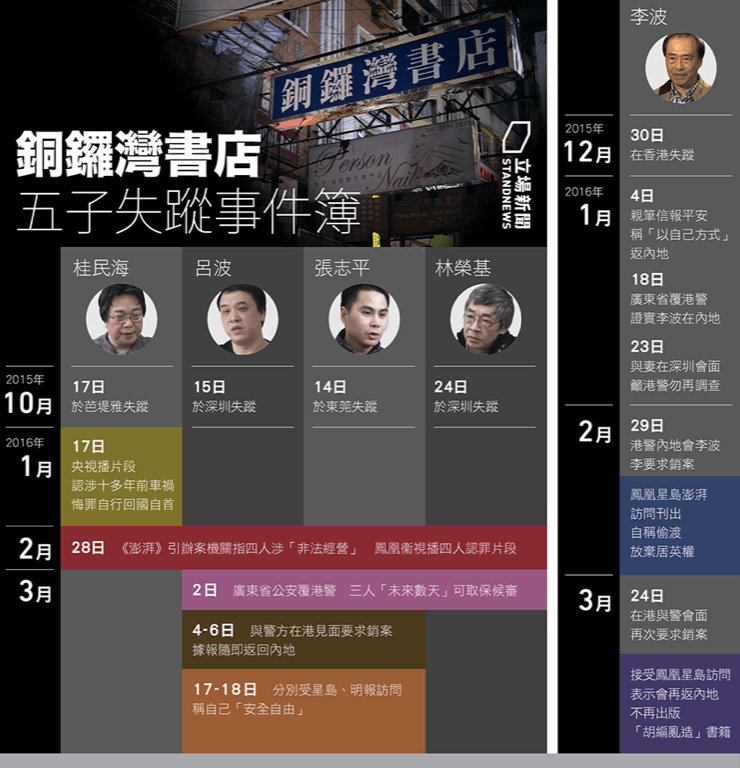
\includegraphics[width=0.7\textwidth]{c30/h-klesson1-048.png}
    \caption{「銅羅灣五子」疑團至今未解} 
\end{figure}

上述各種質疑如果屬實,從法治的角度固然是明顯倒退。就算無法逐一證實各種指控,這些質疑能夠廣泛流傳,本身已是一個嚴重的社會警號。回到政權認授的討論(見問題十四),一個政權如果要靠武力來維持管治,是相當沒有效率和不穩定的。最起碼,被統治者要感到政權對武力的運用及其背後的制度是合理而非隨意,才會自願和政權合作。相反,當被統治者對武力的運用及其背後的制度不再信任,管治成本會大為增加,社會也會變得不穩定。

當公眾都認定政府慣於選擇性執法,各種與執法相關的社會議題都會成為政治問題。例如有農地或舊樓在有業權或發展糾紛的時候剛好發生火警,如果警方未能立即查明真相,則很快便會有人質疑是和發展商相關的人刻意放火生事,然後警方包庇縱容。就算警方查明火警只是意外,也會有人說只是為了掩蓋真相,各種陰謀論流傳不退。這些猜測,都會打擊政府的公信力,使管治變得更為困難。然而拘控「造謠者」只是治標,更重要的是解決政府失信於民的問題。因此,一個正常的政府和一隊正常的警隊,本來是應該盡可能改善警民關係,讓公眾相信警察不偏不倚。

評論人陳雲曾以「如何毀滅一隊警察」為題,指出政府執法失去市民信任的嚴重後果。他提到執法者對以最嚴厲的方式對待抗爭者時時,抗爭不會因而停止,反而變得更極端。如果「示威者稍有異動,都會被控告襲警,反正罪名一樣,為何不真打起來呢?」陳雲這篇文章刊於二零一零年初,很不幸成預視了往後香港的警民關係。

警察地位的改變,後面涉及香港人和特區政府對法治的理解落差。回到港英時代,政府考慮到香港處於冷戰前沿的地緣交界,自戰後逐步建立起對法治的尊重,如對共產黨與國民黨勢力一視同仁地管理,以贏取社會對管治者的信任。面對中國大陸的各式政治運動,法治所強調的制度理性和穩定成為了香港人與中國大陸區分開的重要身分認同依據。來到後九七時期,法治則成為了在沒有全面民主下香港人對抗專制任意性的最後堡壘。這些想法無疑有過度神化和浪漫化的面向,卻曾經在大眾心目中有著至高無上的地位。當對法治的理解從「法律面前人人平等」的價值追求暗暗降格為「總之犯法就不對」的機械式操作,引發的社會震盪自然不可小覷。



伸延閱讀:

吳達明(2002):〈法治的理想與現實〉,謝均才編《我們的地方 我們的時間 香港社會新編》,香港:牛津大學出版社。

陳雲(2010):〈如何毀滅一隊警察〉,《信報》2010年1月26日

蔡俊威,李家翹(2018):〈假戲真做 弄假成真 政治的法律化:法治作為意識形態〉,《明報》2018年10月14日。

網上資源:

\href{http://www.thestand.news/politics/銅鑼灣書店五子失蹤事件簿/}{立場報道(2016)銅鑼灣書店五子失蹤事件簿,2016年3月24日}

\href{https://thestandnews.com/society/紀律部隊民調續包尾-警隊滿意淨值急插-史上第二低/}{立場報道(2018)紀律部隊民調 警隊續包尾 滿意淨值急插 史上第二低,2018年6月5日}